\section{Physical Elements}
In this section we will go through the different iterations that the track and bus have gone through. We will end each subsection with a picture showing its final version.

\subsection{Track}
The first designed track can be seen in figure \ref{Track1Layout}. The layout of the track is quite simple and only contain some of the requirements described in section \ref{Requirements}. This is a limited design made to test early versions of the bus. The lane width and radius of the turn we determined based on the maximal turning angle of the current bus, shown in Figure \ref{bus1Design}.

\begin{figure}[H]
    \centering
    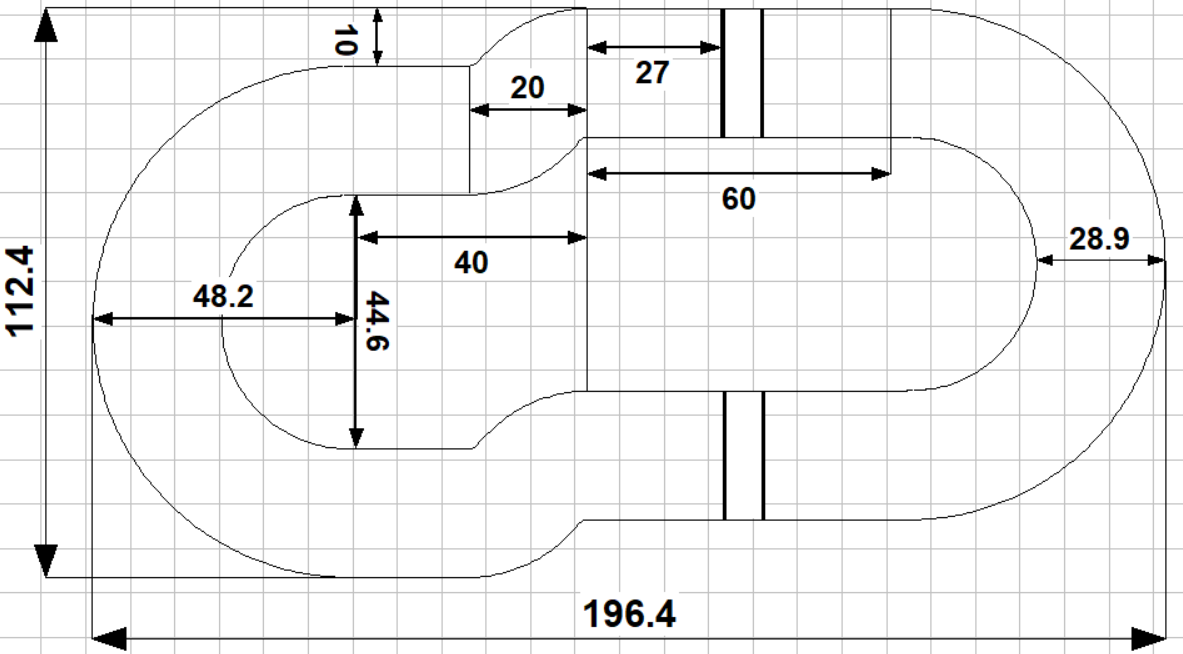
\includegraphics[width=0.8\textwidth]{Images/Tracks/Track1.PNG}
    \caption{Initial track Layout given in cm}
    \label{Track1Layout}
\end{figure}

Using this design we made the following track by taping sheets of paper together and adding the black tape according to the design. which resulted in the following track shown in Figure \todo{add ref}
The track is quite similar to the first track, however in this iteration the track contains a bus stop, and it is a loop. Furthermore the aspect ratio have been changed slightly to fit the redesigned bus.

\begin{figure}[H]
    \centering
    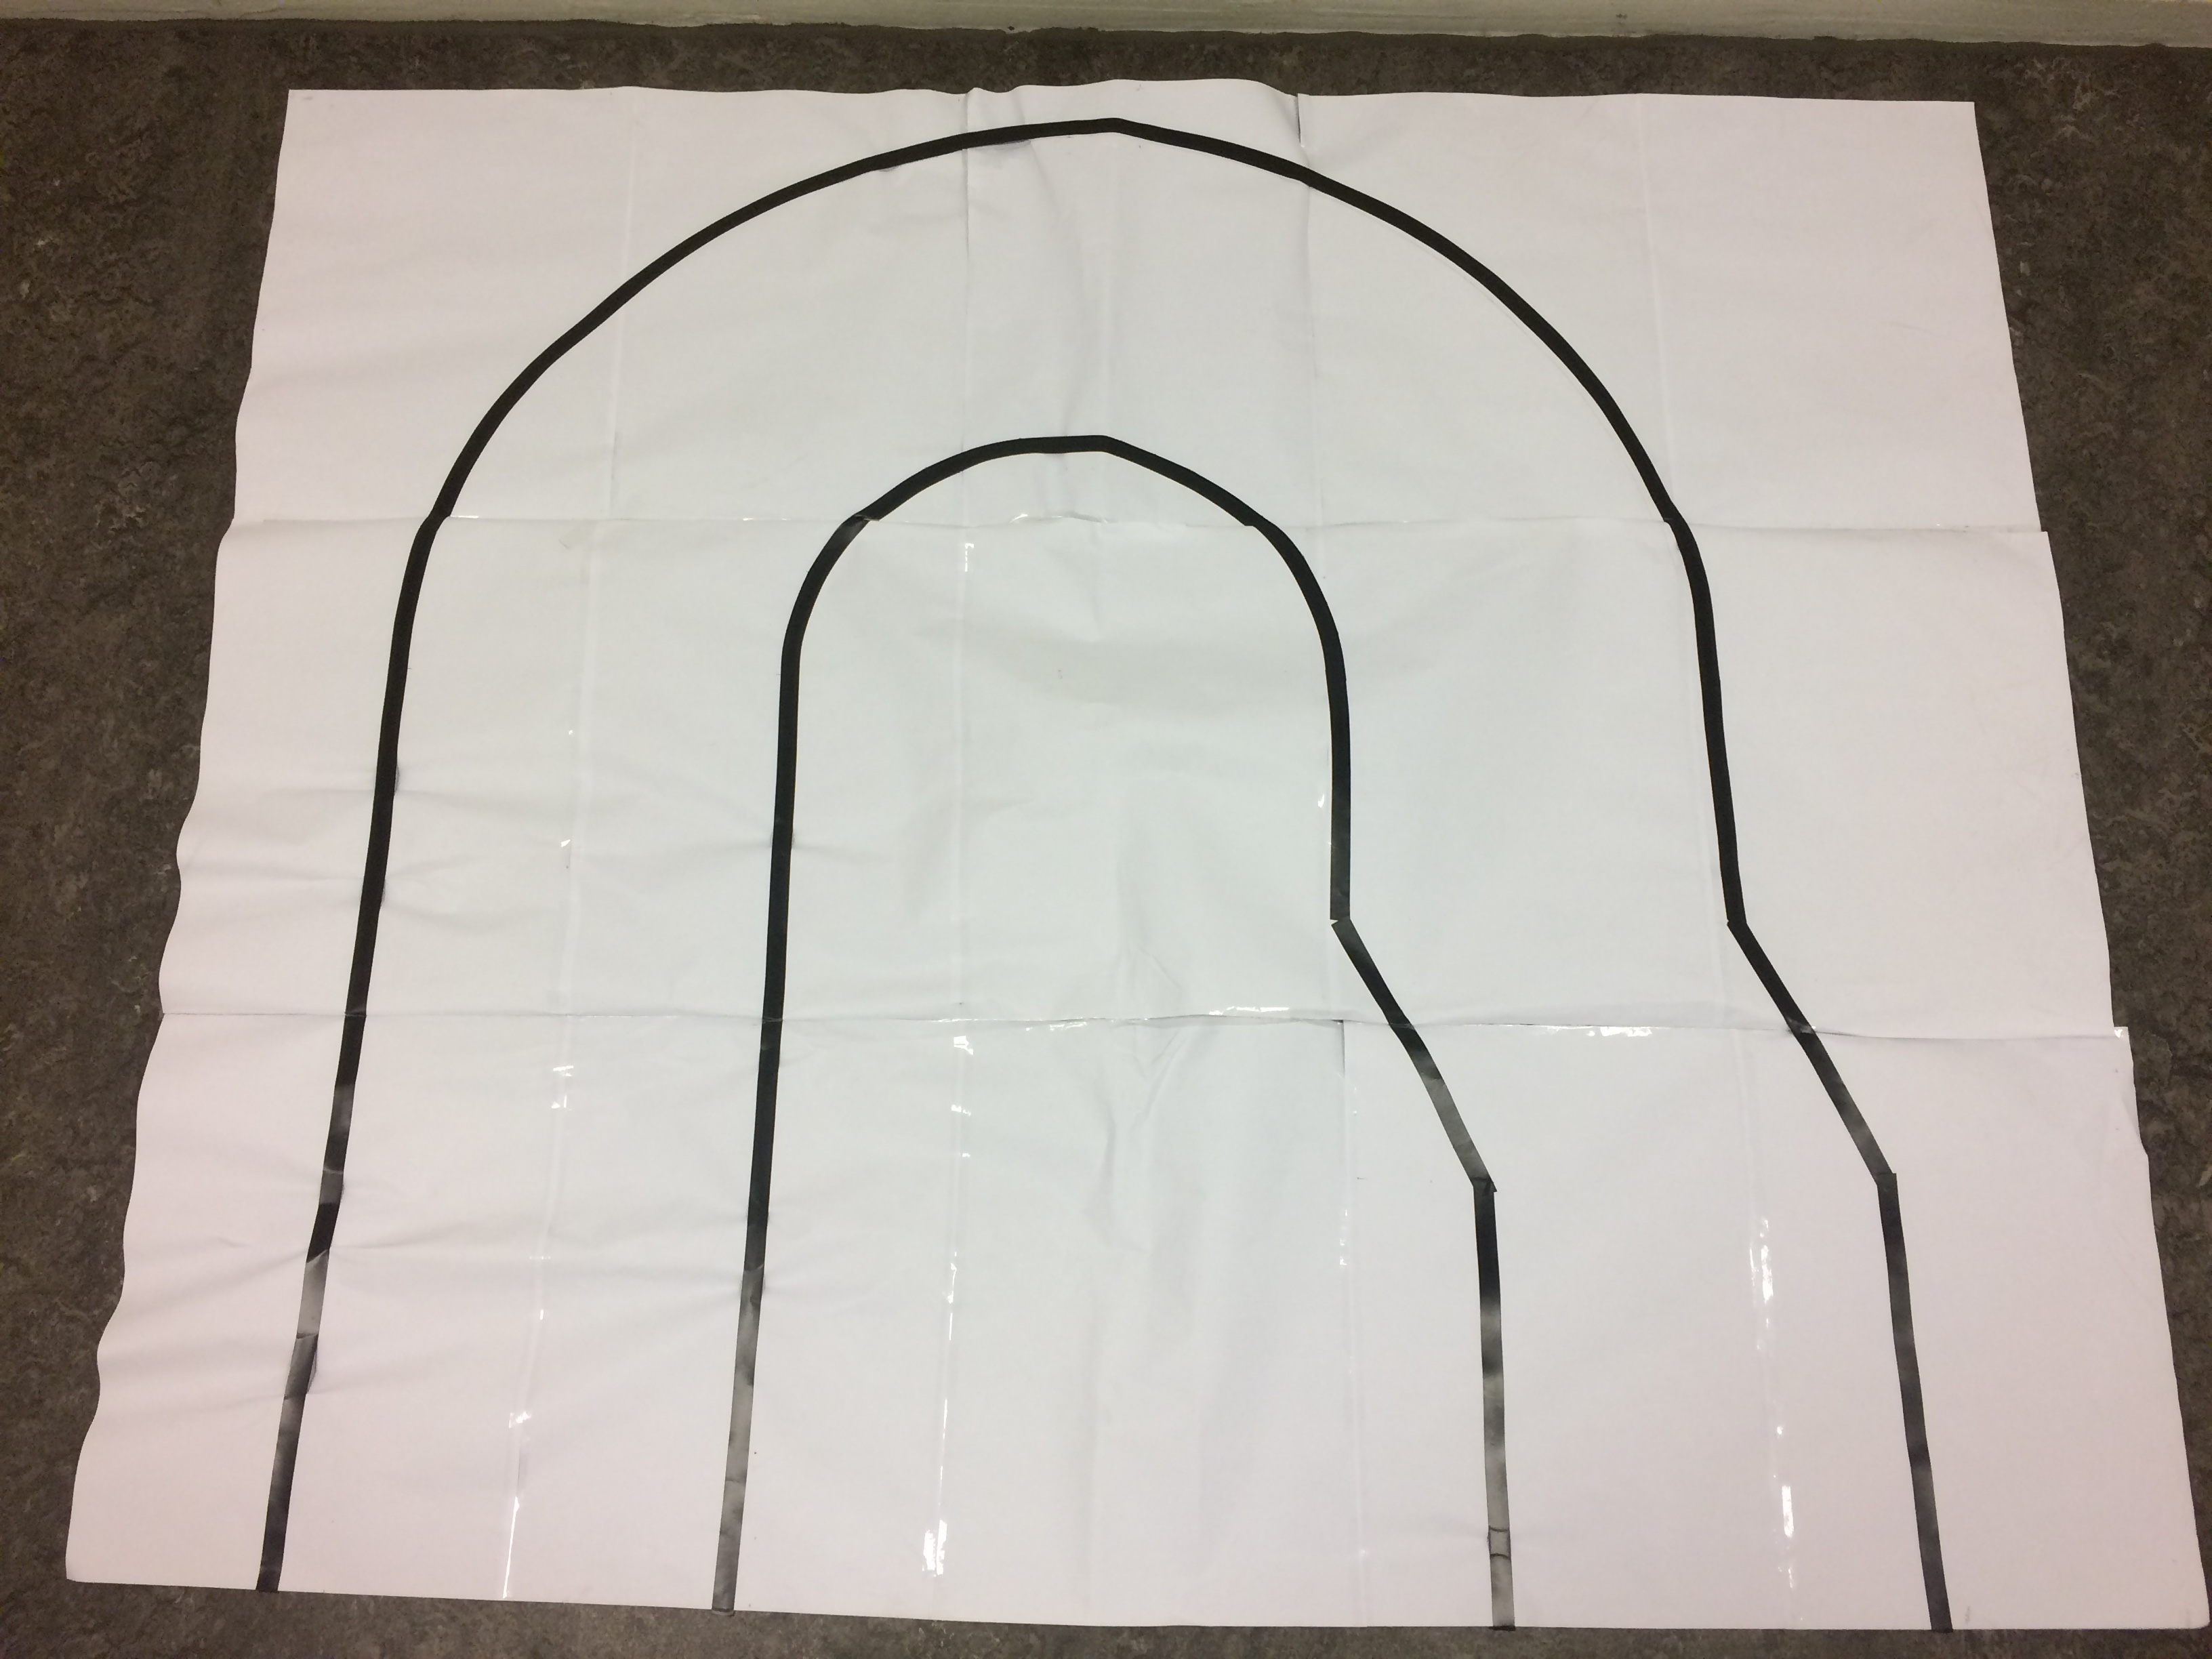
\includegraphics[width=0.8\textwidth]{Images/Tracks/initialTrack.jpg}
    \caption{Initial track picture}
    \label{initalTraclLayout}
\end{figure}
%Figure

However there were some problems that that occurred because of how the track were made. The paper would bobble up the places where it was taped together making both the ultrasound and NXTCam's data more unreliable. And it was hard to carry and store.

So another method had to be found to use when creating the final track, fortunately we were given the idea to use tablecloth when creating our track. With this and the design described in \ref{trackDesign} the track shown in Figure \ref{FinalTrackLayout} was made.

\begin{figure}[H]
    \centering
    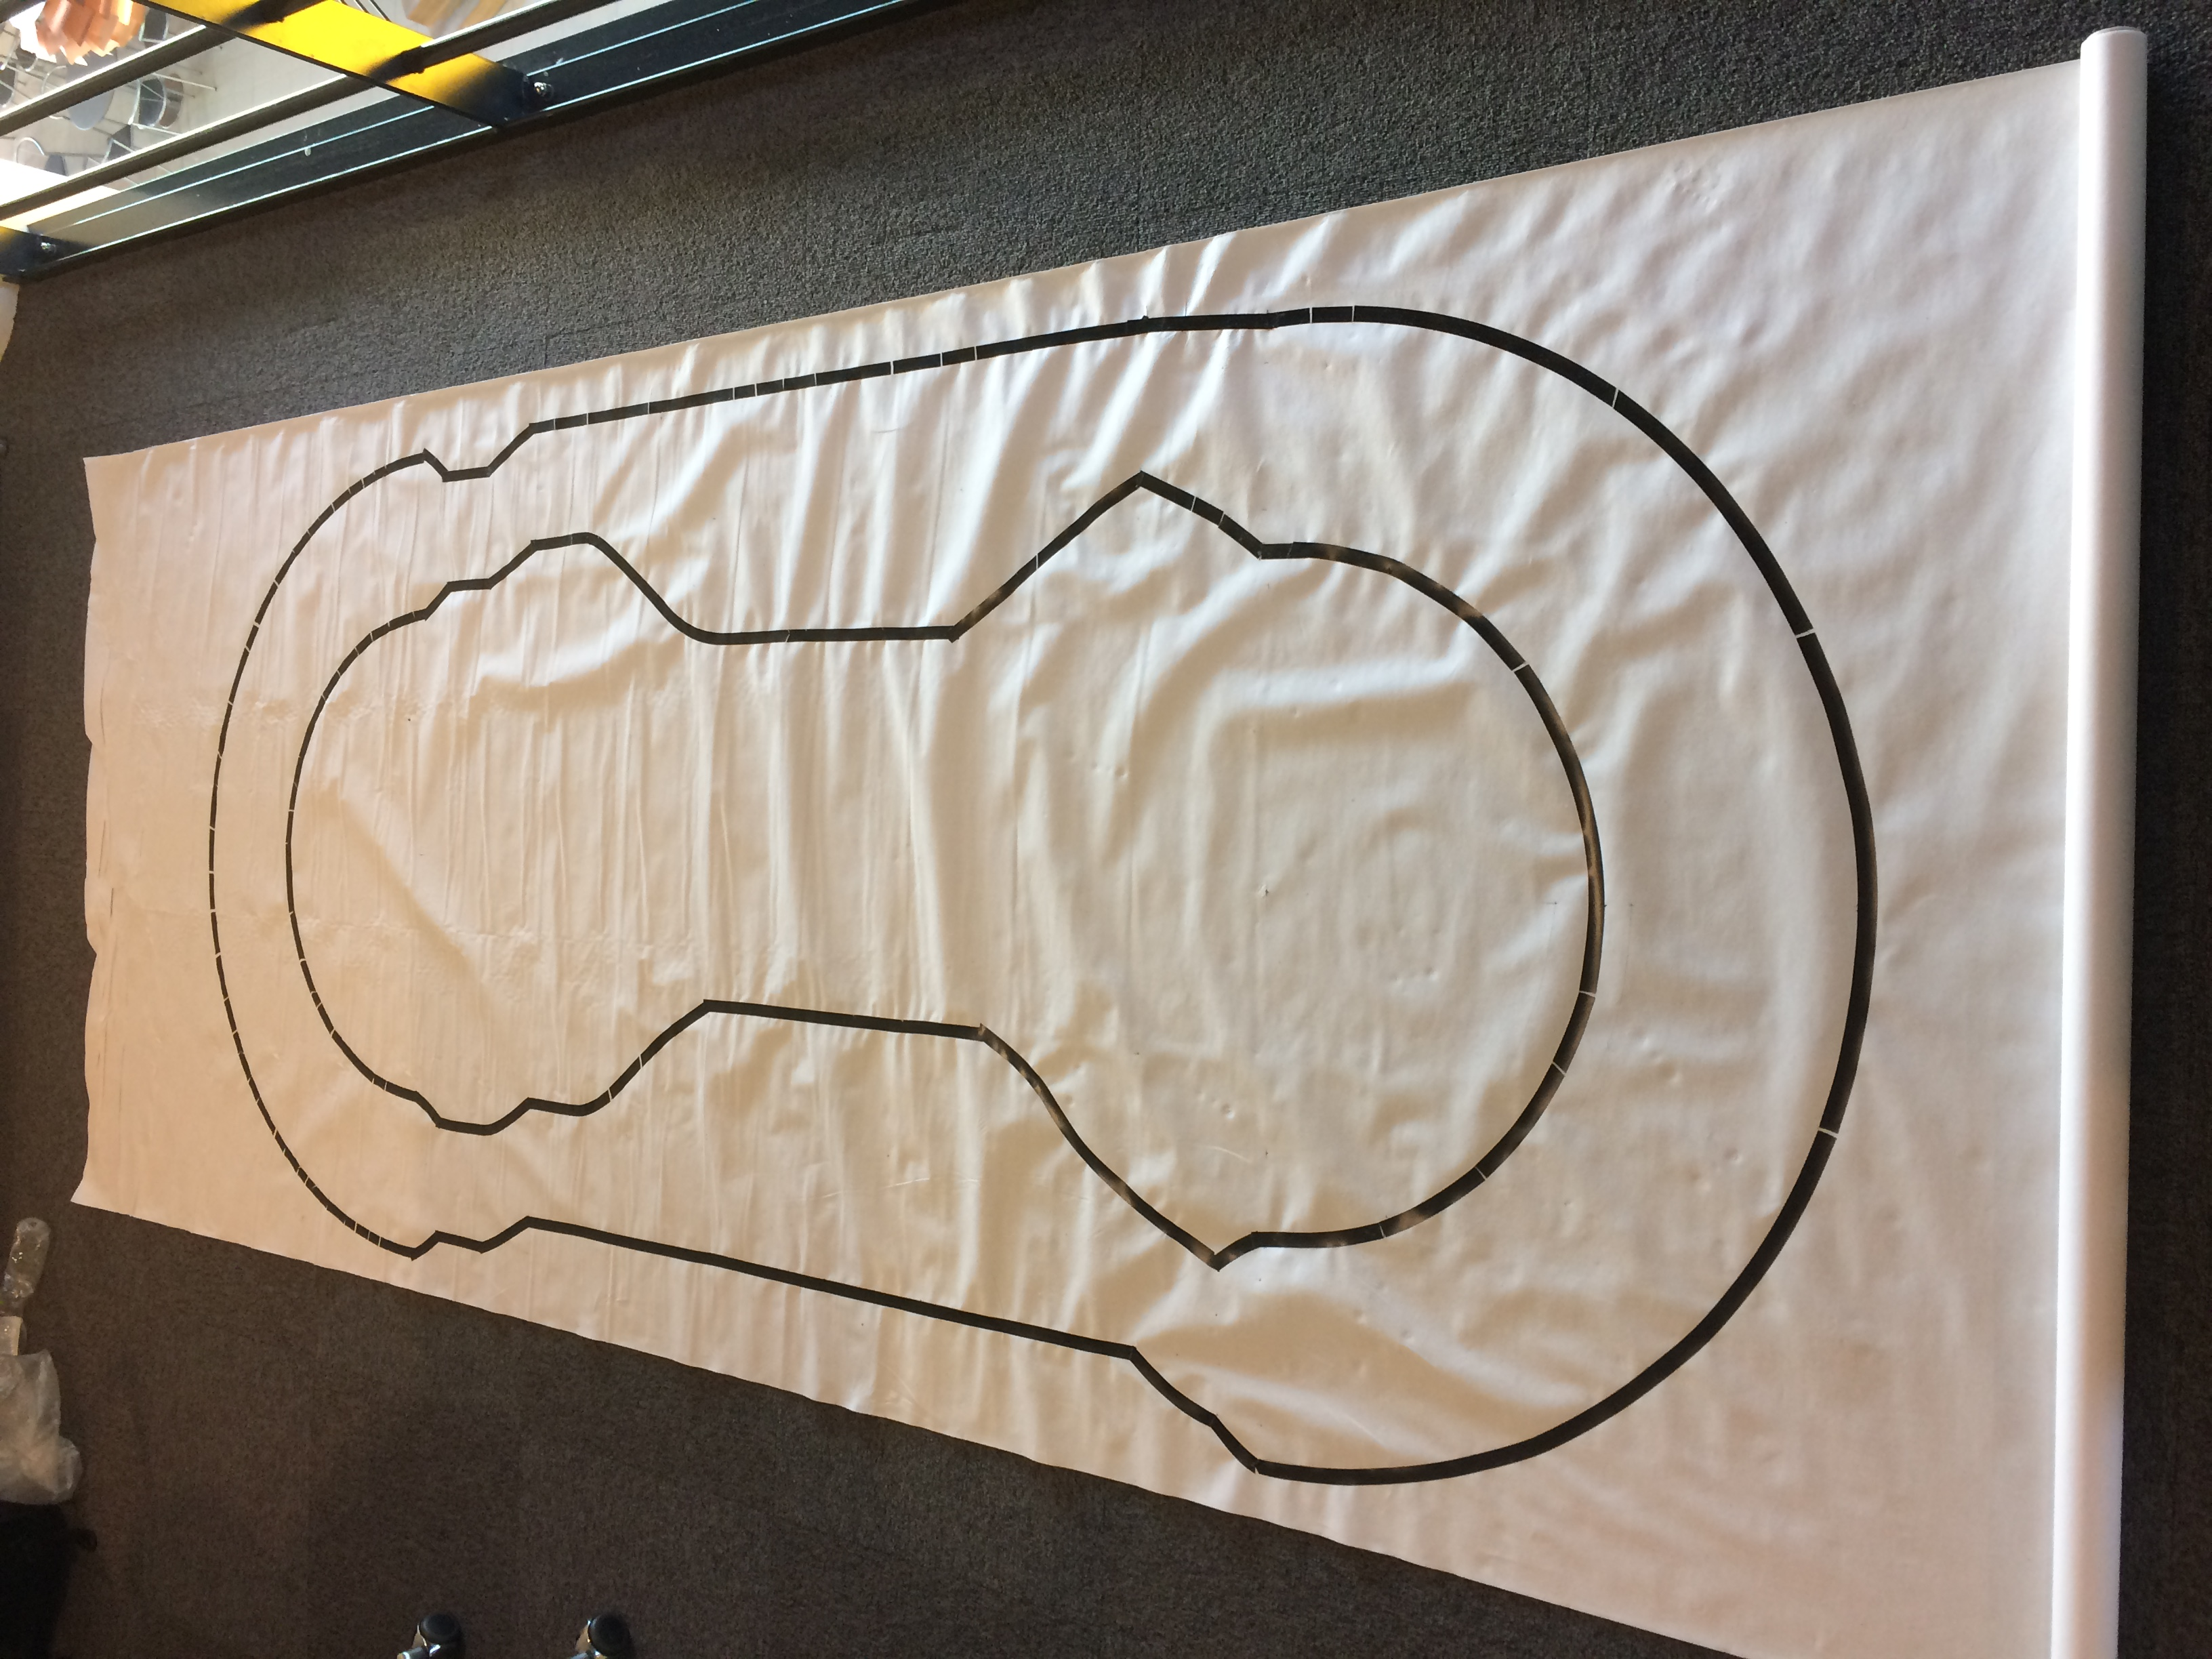
\includegraphics[width=0.8\textwidth, angle=270]{Images/Tracks/FinalTrack.jpg}
    \caption{Final track picture}
    \label{FinalTrackLayout}
\end{figure}
%Figure

\subsection{Bus}
To start of we focused on simply having a vehicle on which we were able to test simple code on, a prototype designed solely for this purpose is built. The prototype needs to be able to drive, turn and brake. For this purpose we created the vehicle shown in Figure \ref{bus1Design}.

\begin{figure}[H]
    \centering
    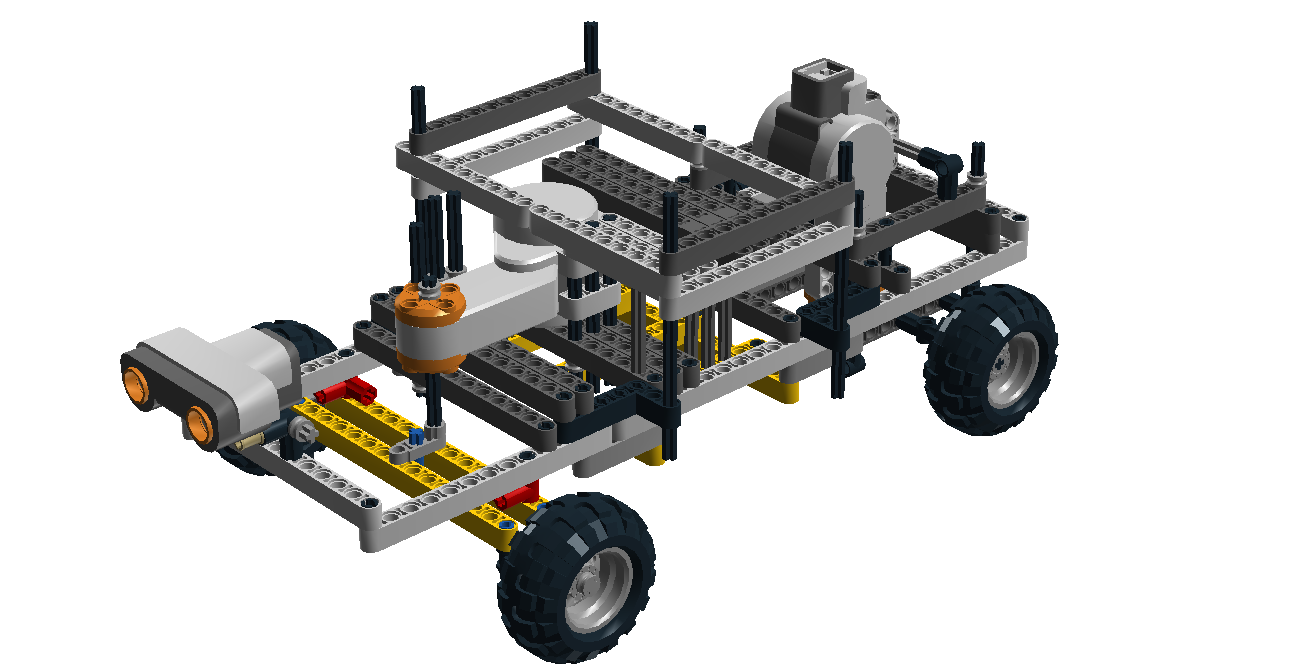
\includegraphics[width=0.8\textwidth]{Images/implementation/6.png}
    \caption{Initial bus design}
    \label{bus1Design}
\end{figure}


However this implementation was not without problems. It would sometimes lose its wheels and were easily damaged so we made the bus shown in Figure \ref{CrazyGood}.

\begin{figure}[H]
    \centering
    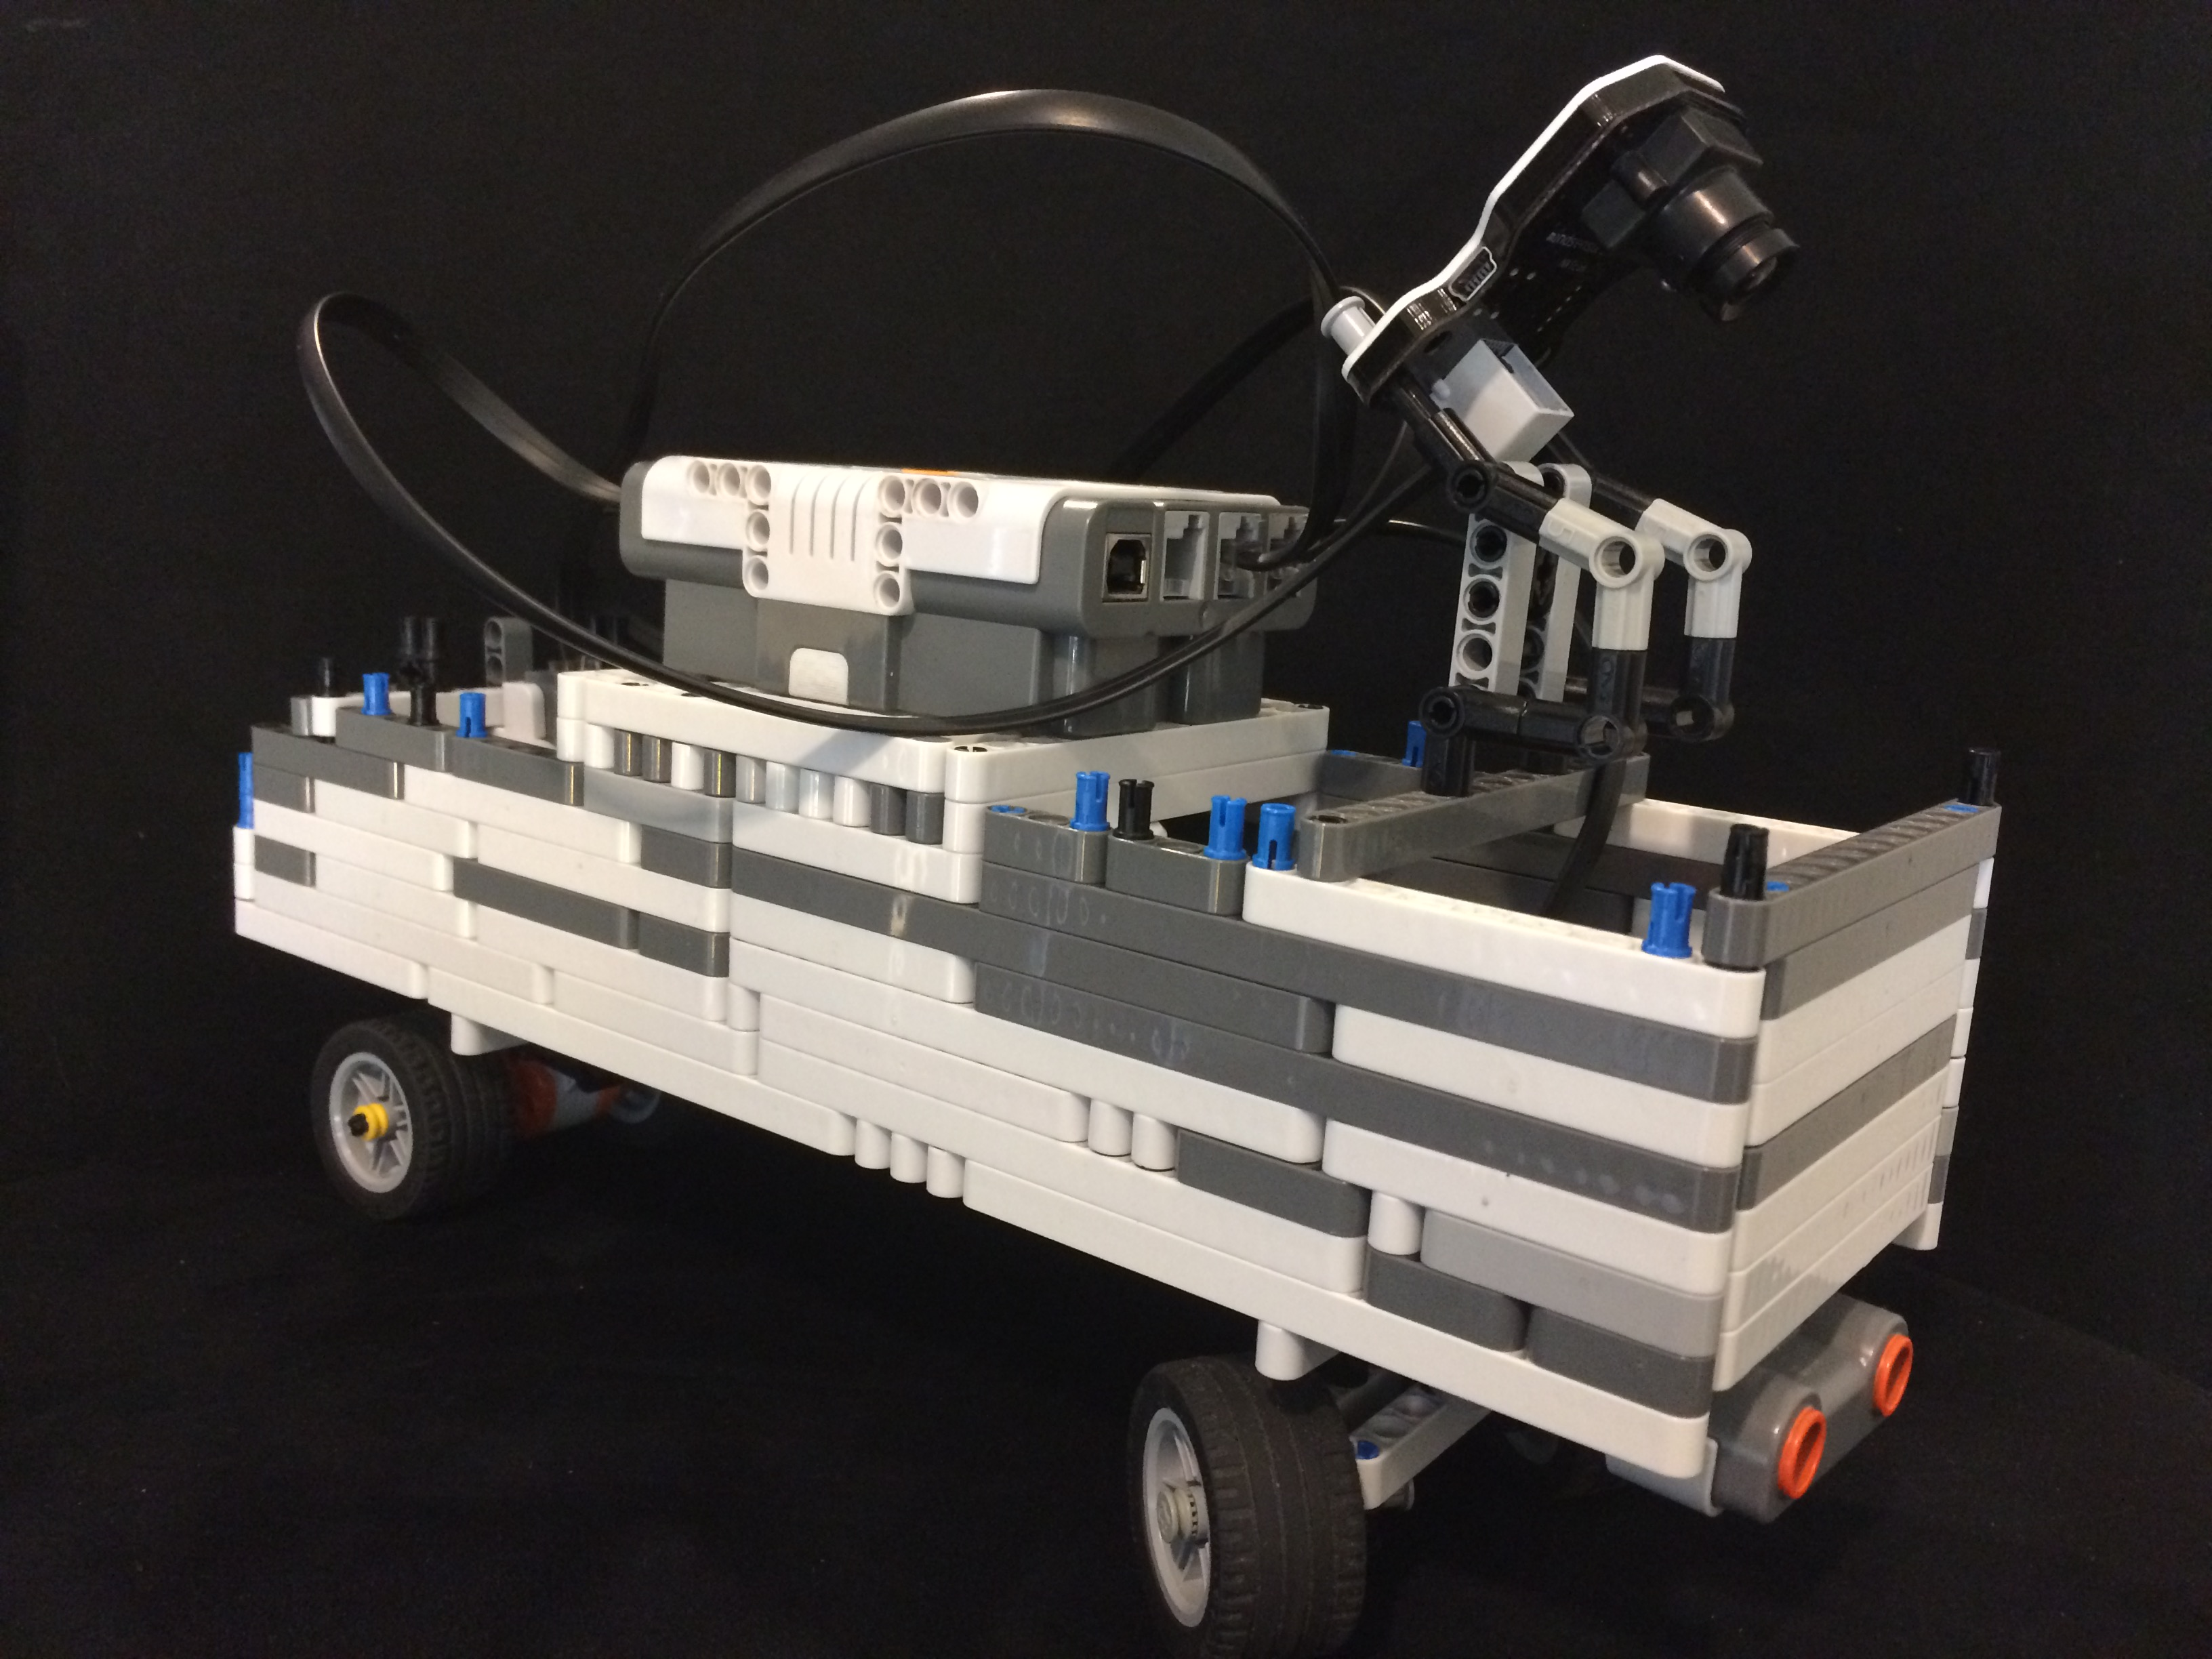
\includegraphics[width=0.8\textwidth]{Images/implementation/CrazzzyGoodPictureBus.jpg}
    \caption{Final bus design}
    \label{CrazyGood}
\end{figure}
